\chapter{Appendix A} \label{cp:figures}

\section{Additional Apparatus Pictures} \label{sec:additional_apparatus}

\begin{figure}[htpb]
    \centering
    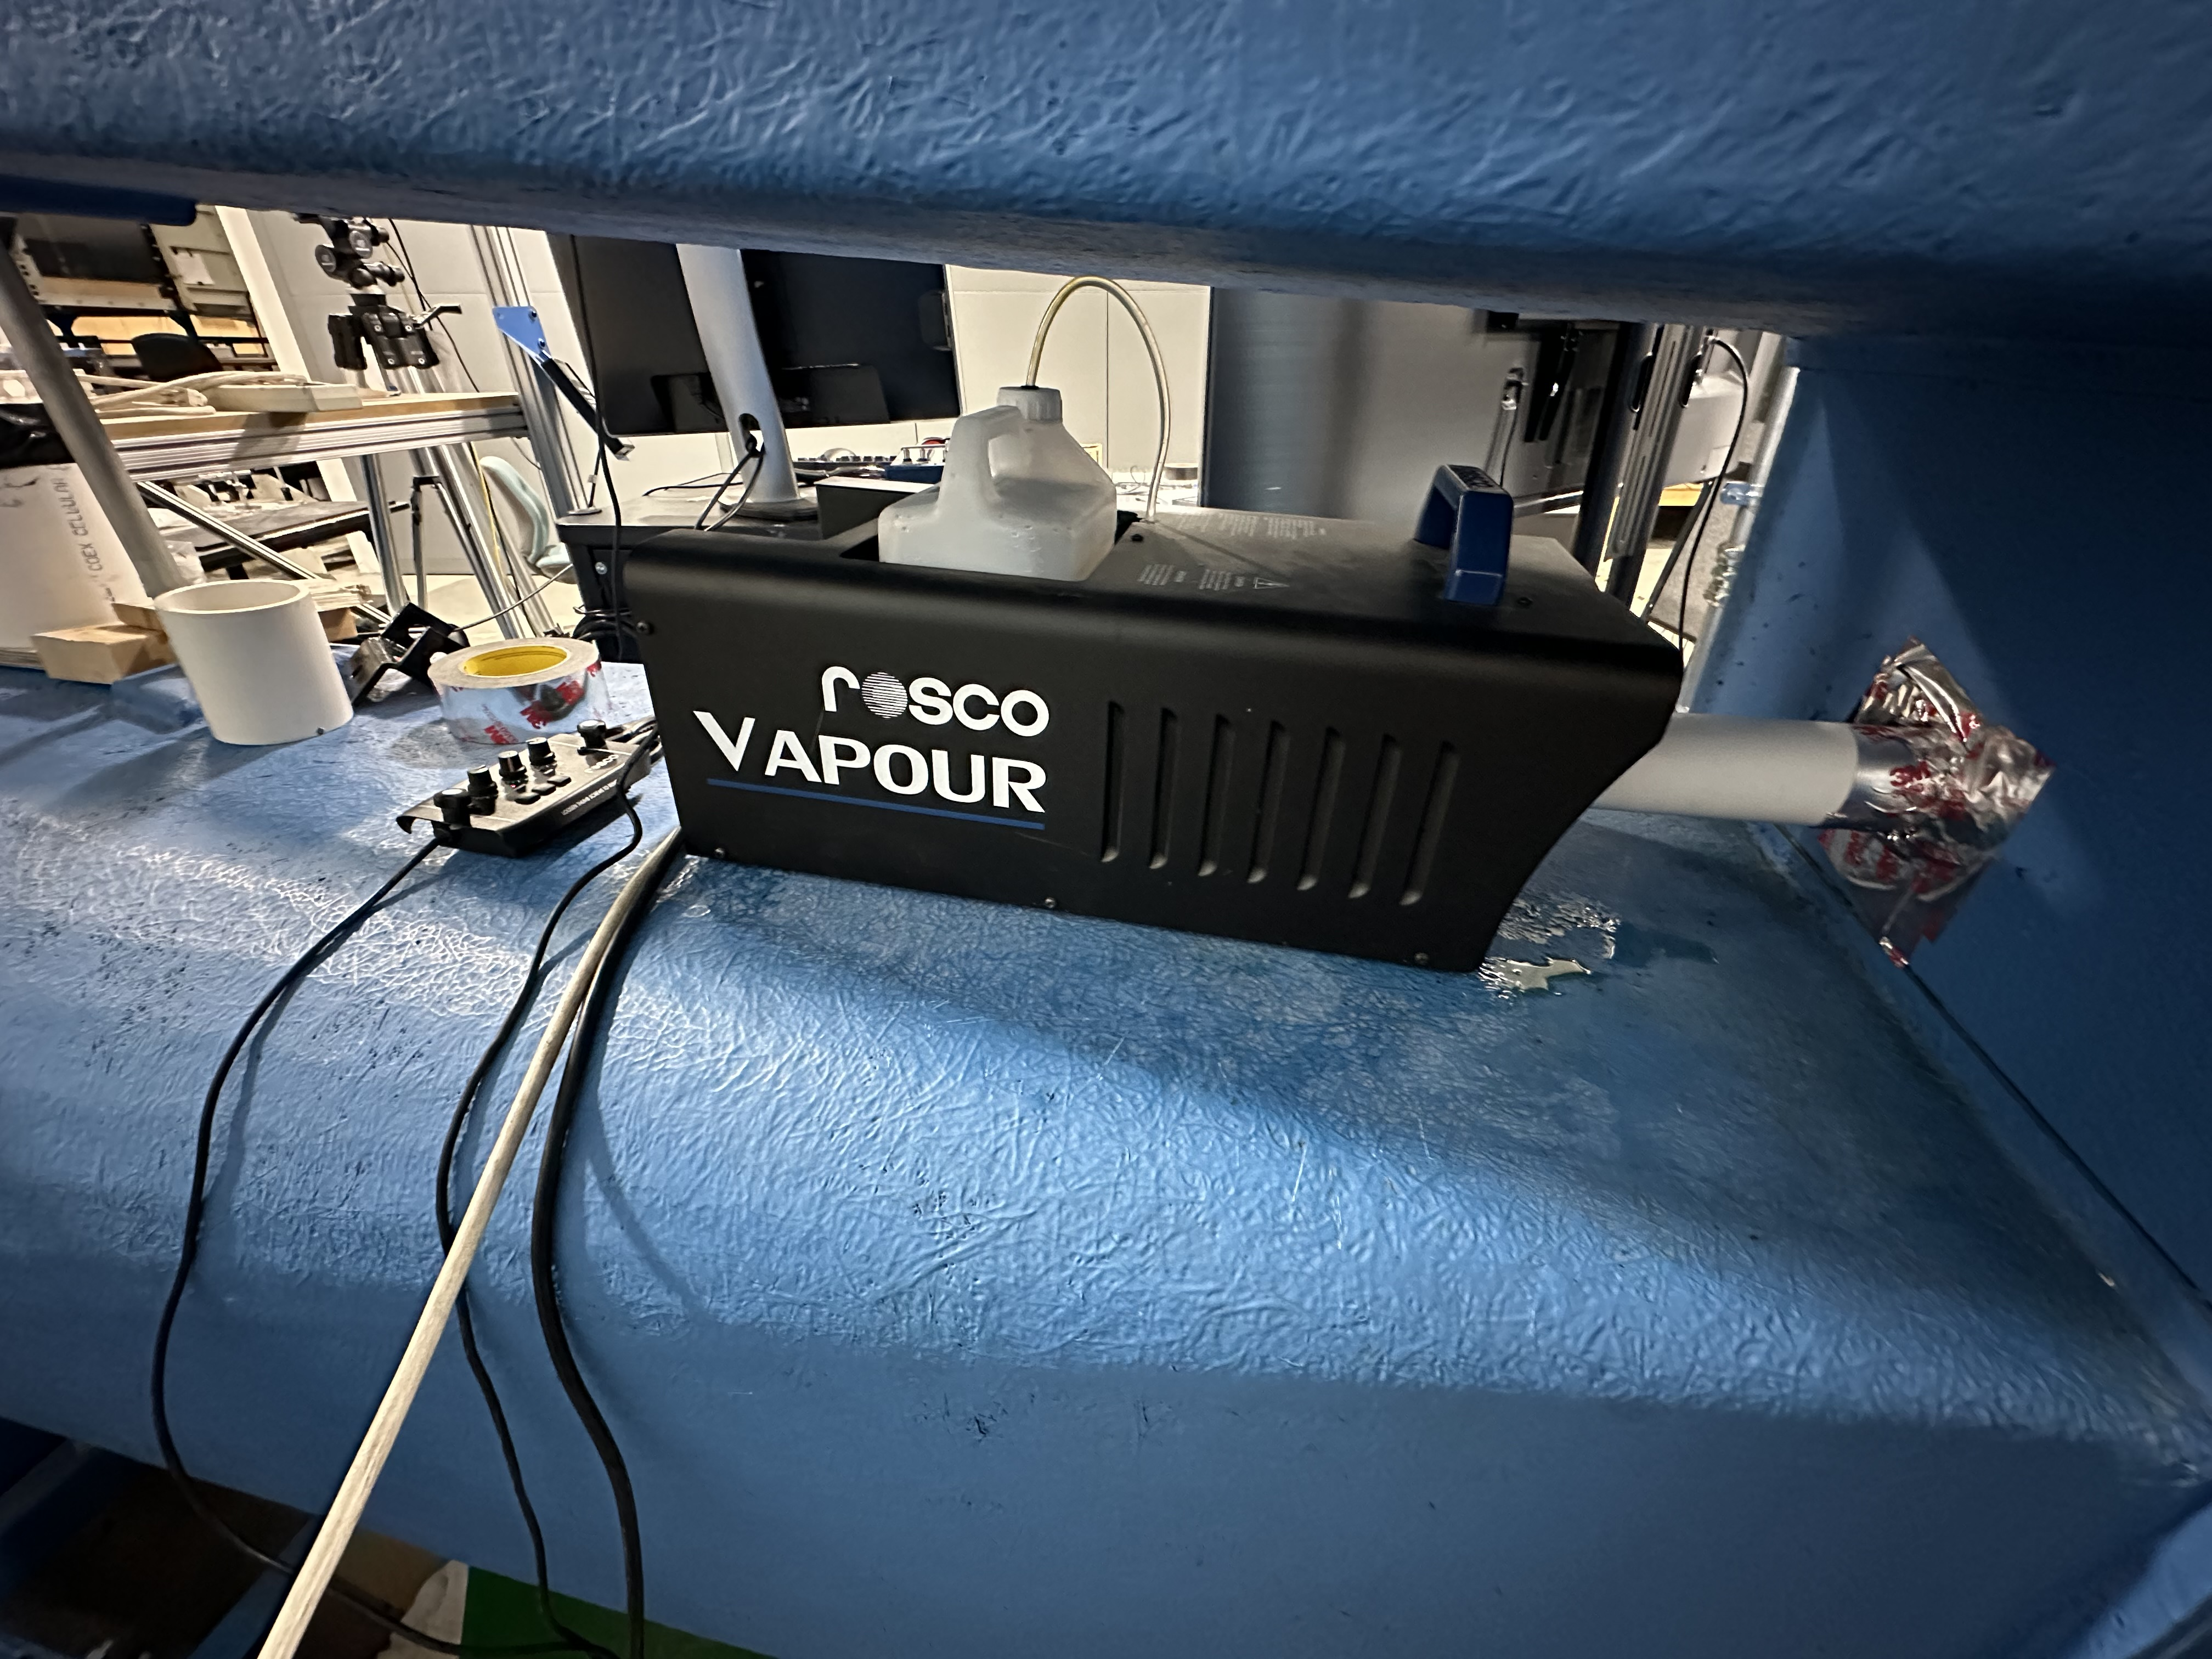
\includegraphics[width=\linewidth]{Figures/IMG_0135.jpeg}
    \caption{The smoke machine.}
    \label{fig:smoke_machine}
\end{figure}

\begin{figure}[htpb]
    \centering
    \includegraphics[width=\linewidth]{Figures/IMG_0136.jpeg}
    \caption{The delay generator.}
    \label{fig:delay_generator}
\end{figure}

\begin{figure}[htpb]
    \centering
    \includegraphics[width=\linewidth]{Figures/IMG_0137.jpeg}
    \caption{The laser generator.}
    \label{fig:laser_generator}
\end{figure}

\newpage
\section{Full Size Figures} \label{sec:full_size_figures}

\begin{figure}[htpb]
    \centering
    \includesvg[width=\linewidth]{Figures/Instantaneous PIV Measurements - AOA8.svg}
    \caption{The instantaneous velocity vector field and vorticity distribution for data frame \num{202} at \qty{8}{\degree} \acrshort{aoa}.}
    \label{fig:full_instant_aoa8}
\end{figure}

\begin{figure}[htpb]
    \centering
    \includesvg[width=0.95\linewidth]{Figures/Instantaneous PIV Measurements - AOA16.svg}
    \caption{The instantaneous velocity vector field and vorticity distribution for data frame \num{245} at \qty{16}{\degree} \acrshort{aoa}.}
    \label{fig:full_instant_aoa16}
\end{figure}

\begin{figure}[htpb]
    \centering
    \includesvg[width=\linewidth]{Figures/Ensemble PIV Measurements - AOA4.svg}
    \caption{The averaged velocity vector field and vorticity distribution at \qty{4}{\degree} \acrshort{aoa}.}
    \label{fig:full_averaged_piv_aoa4}
\end{figure}

\begin{figure}[htpb]
    \centering
    \includesvg[width=\linewidth]{Figures/Ensemble PIV Measurements - AOA8.svg}
    \caption{The averaged velocity vector field and vorticity distribution at \qty{8}{\degree} \acrshort{aoa}.}
    \label{fig:full_averaged_piv_aoa8}
\end{figure}

\begin{figure}[htpb]
    \centering
    \includesvg[width=\linewidth]{Figures/Ensemble PIV Measurements - AOA12.svg}
    \caption{The averaged velocity vector field and vorticity distribution at \qty{12}{\degree} \acrshort{aoa}.}
    \label{fig:full_averaged_piv_aoa12}
\end{figure}

\begin{figure}[htpb]
    \centering
    \includesvg[width=\linewidth]{Figures/Ensemble PIV Measurements - AOA16.svg}
    \caption{The averaged velocity vector field and vorticity distribution at \qty{16}{\degree} \acrshort{aoa}.}
    \label{fig:full_averaged_piv_aoa16}
\end{figure}

\begin{figure}[htpb]
    \centering
    \includesvg[width=\linewidth]{Figures/Ensemble Turbulent Kinetic Energy - AOA4.svg}
    \caption{The averaged turbulent kinetic energy distribution at \qty{4}{\degree} \acrshort{aoa}.}
    \label{fig:full_averaged_ke_aoa4}
\end{figure}

\begin{figure}[htpb]
    \centering
    \includesvg[width=\linewidth]{Figures/Ensemble Turbulent Kinetic Energy - AOA8.svg}
    \caption{The averaged turbulent kinetic energy distribution at \qty{8}{\degree} \acrshort{aoa}.}
    \label{fig:full_averaged_ke_aoa8}
\end{figure}

\begin{figure}[htpb]
    \centering
    \includesvg[width=\linewidth]{Figures/Ensemble Turbulent Kinetic Energy - AOA12.svg}
    \caption{The averaged turbulent kinetic energy distribution at \qty{12}{\degree} \acrshort{aoa}.}
    \label{fig:full_averaged_ke_aoa12}
\end{figure}

\begin{figure}[htpb]
    \centering
    \includesvg[width=\linewidth]{Figures/Ensemble Turbulent Kinetic Energy - AOA16.svg}
    \caption{The averaged turbulent kinetic energy distribution at \qty{16}{\degree} \acrshort{aoa}.}
    \label{fig:full_averaged_ke_aoa16}
\end{figure}

\begin{figure}[htpb]
    \centering
    \includesvg[width=\linewidth]{Figures/Wake Profile at Half Chord Downstream - AOA4.svg}
    \caption{The velocity magnitude profile at half chord for \qty{4}{\degree} \acrshort{aoa}.}
    \label{fig:full_averaged_half_chord_aoa4}
\end{figure}

\begin{figure}[htpb]
    \centering
    \includesvg[width=\linewidth]{Figures/Wake Profile at Half Chord Downstream - AOA8.svg}
    \caption{The velocity magnitude profile at half chord for \qty{8}{\degree} \acrshort{aoa}.}
    \label{fig:full_averaged_half_chord_aoa8}
\end{figure}

\begin{figure}[htpb]
    \centering
    \includesvg[width=\linewidth]{Figures/Wake Profile at Half Chord Downstream - AOA12.svg}
    \caption{The velocity magnitude profile at half chord for \qty{12}{\degree} \acrshort{aoa}.}
    \label{fig:full_averaged_half_chord_aoa12}
\end{figure}

\begin{figure}[htpb]
    \centering
    \includesvg[width=\linewidth]{Figures/Wake Profile at Half Chord Downstream - AOA16.svg}
    \caption{The velocity magnitude profile at half chord for \qty{16}{\degree} \acrshort{aoa}.}
    \label{fig:full_averaged_half_chord_aoa16}
\end{figure}